% !TEX root = ../main.tex
\newpage
\section{\mywork Emerging Network Topologies}
%\textcolor{red}{TODO}: \textsl{explain in detail how the different methods \cref{eq:KempterSTDPFormulation2,eq:SongSTDPFormulation} will be implemented, using \STDP coupled with \IP.}

We will now investigate what topologies emerge from the learning procedures described in Chapter \ref{sec:HebbianLearningAndSynapticPlasticity}. Are the approaches presented in \cite{Kempter1999, Song2000, Song2017, ChrolCannon2012} plausible within the context of the Theta model? Do we obtain similar results concerning synchronisation and topology? Is there a reason for only allowing the network to make excitatory ($K_{ij} \geq 0$) connections? 

\subsection{Conditions of the network}
As we saw in Chapter \ref{sec:MFRs}, the typical range for the coupling strength $\kappa$ and the mean excitability $\eta_0$ to alter the macroscopic state of the network drastically is fairly large. Using the Kempter method \eqref{eq:KempterSTDPFormulation2}, there is no limit on the magnitude of $K$, and convergence of the node degrees was observed within the interval [-100, 100]. 

When using the Song method \eqref{eq:SongSTDPFormulation} we will constrain $-K^{\rm max} \leq K_{ij} \leq K^{\rm max}$ to allow neurons to both exhibit exitatory and inhibitory behaviour. When testing different values of $K^{\rm max}$ no significant difference was observed in the results, except the time of reaching convergence of $\kmean$. To optimally compare the two methods we will use $K^{\rm max}$ = 100. $K_{ij}$ is always initialised using a uniform distribution over $[-K^{\rm max}, K^{\rm max}]$, as to minimise influence of the initial distribution on the resulting topology.\\

The networks we will study consist of 100 Theta neurons, as the computational task of numerically solving the learning equations until convergence is a heavy one. The networks will be initialised with $\theta_i$ equidistantly distributed over $\T$, so that $| Z(0) |$ = 0 exactly. The excitabilities $\eta_i$ are set to zero for all neurons. 
When investigating \STDP + \IP, the excitability is allowed to change over the same domain as $K_{ij}$, in accordance to our comments on $\eta_i$ and $I_i$ cancelling each other out. Therefore we take $\eta_{\max} = K^{\rm max}$ and just like $K_{ij}$, $\eta_i$ is using a uniform distribution over $[-\eta_{\max}, \eta_{\max}]$.


\subsection{Tuning hyperparameters for \texorpdfstring{$W_K$}{TEXT}}
We decided to scale all learning windows presented in Chapter \ref{sec:HebbianLearningAndSynapticPlasticity} to the same order of magnitude, to make for a fair comparison of the learning dynamics over time. What is left now is to tune the hyperparameters $w^{\mathrm{in}}$ and $w^{\mathrm{out}}$. Looking at Figure \ref{fig:KempterWinWout}, we can see that we cannot simply use the same magnitude as the learning window: the dynamics are disturbed by the large discrete changes induced by $w^{\mathrm{in}}$ and $w^{\mathrm{out}}$. A better solution is obtained by using $w^{\mathrm{in}}$ = 10$^{-3}$.

\begin{figure}[H]
\centering
\includegraphics[width = \textwidth]{../Figures/Learning/KempterWinWout.pdf}
\caption{Tuning of the hyperparameters $w^{\mathrm{in}}$ and $w^{\mathrm{out}} = -1.0475 \cdot w^{\mathrm{in}}$. The radius of the order parameter is initialised as zero and quickly becomes non-zero. When neurons start bursting we can see a big drop in synchronisation, and a large increase in $\k$, meaning that the \STDP method works. Left: the learning dynamics with zero weights, as a benchmark. Middle: the learning dynamics for small, non-zero weights. The mean coupling strength is higher, but the overall synchronisation is lower. This might yield an interesting topological structure. Right: the learning dynamics with the same magnitude as the learning window disturb the learning process.}
\label{fig:KempterWinWout}
\end{figure}


\subsection{Results of using \STDP} %applied to networks of theta neurons
We can now use the Kempter method and its corresponding learning window and compare it to the Song method and the bi- and triphasic learning windows. The results are shown in Figure \ref{fig:STDP}.

In the first row of plots, we can see the overall synchronisation of the network and its mean node degree as it learns over time. The Kempter method does not seem to converge


\subsection{Results of using \STDP + \IP}

\newpage
\begin{figure}[H]
\centering
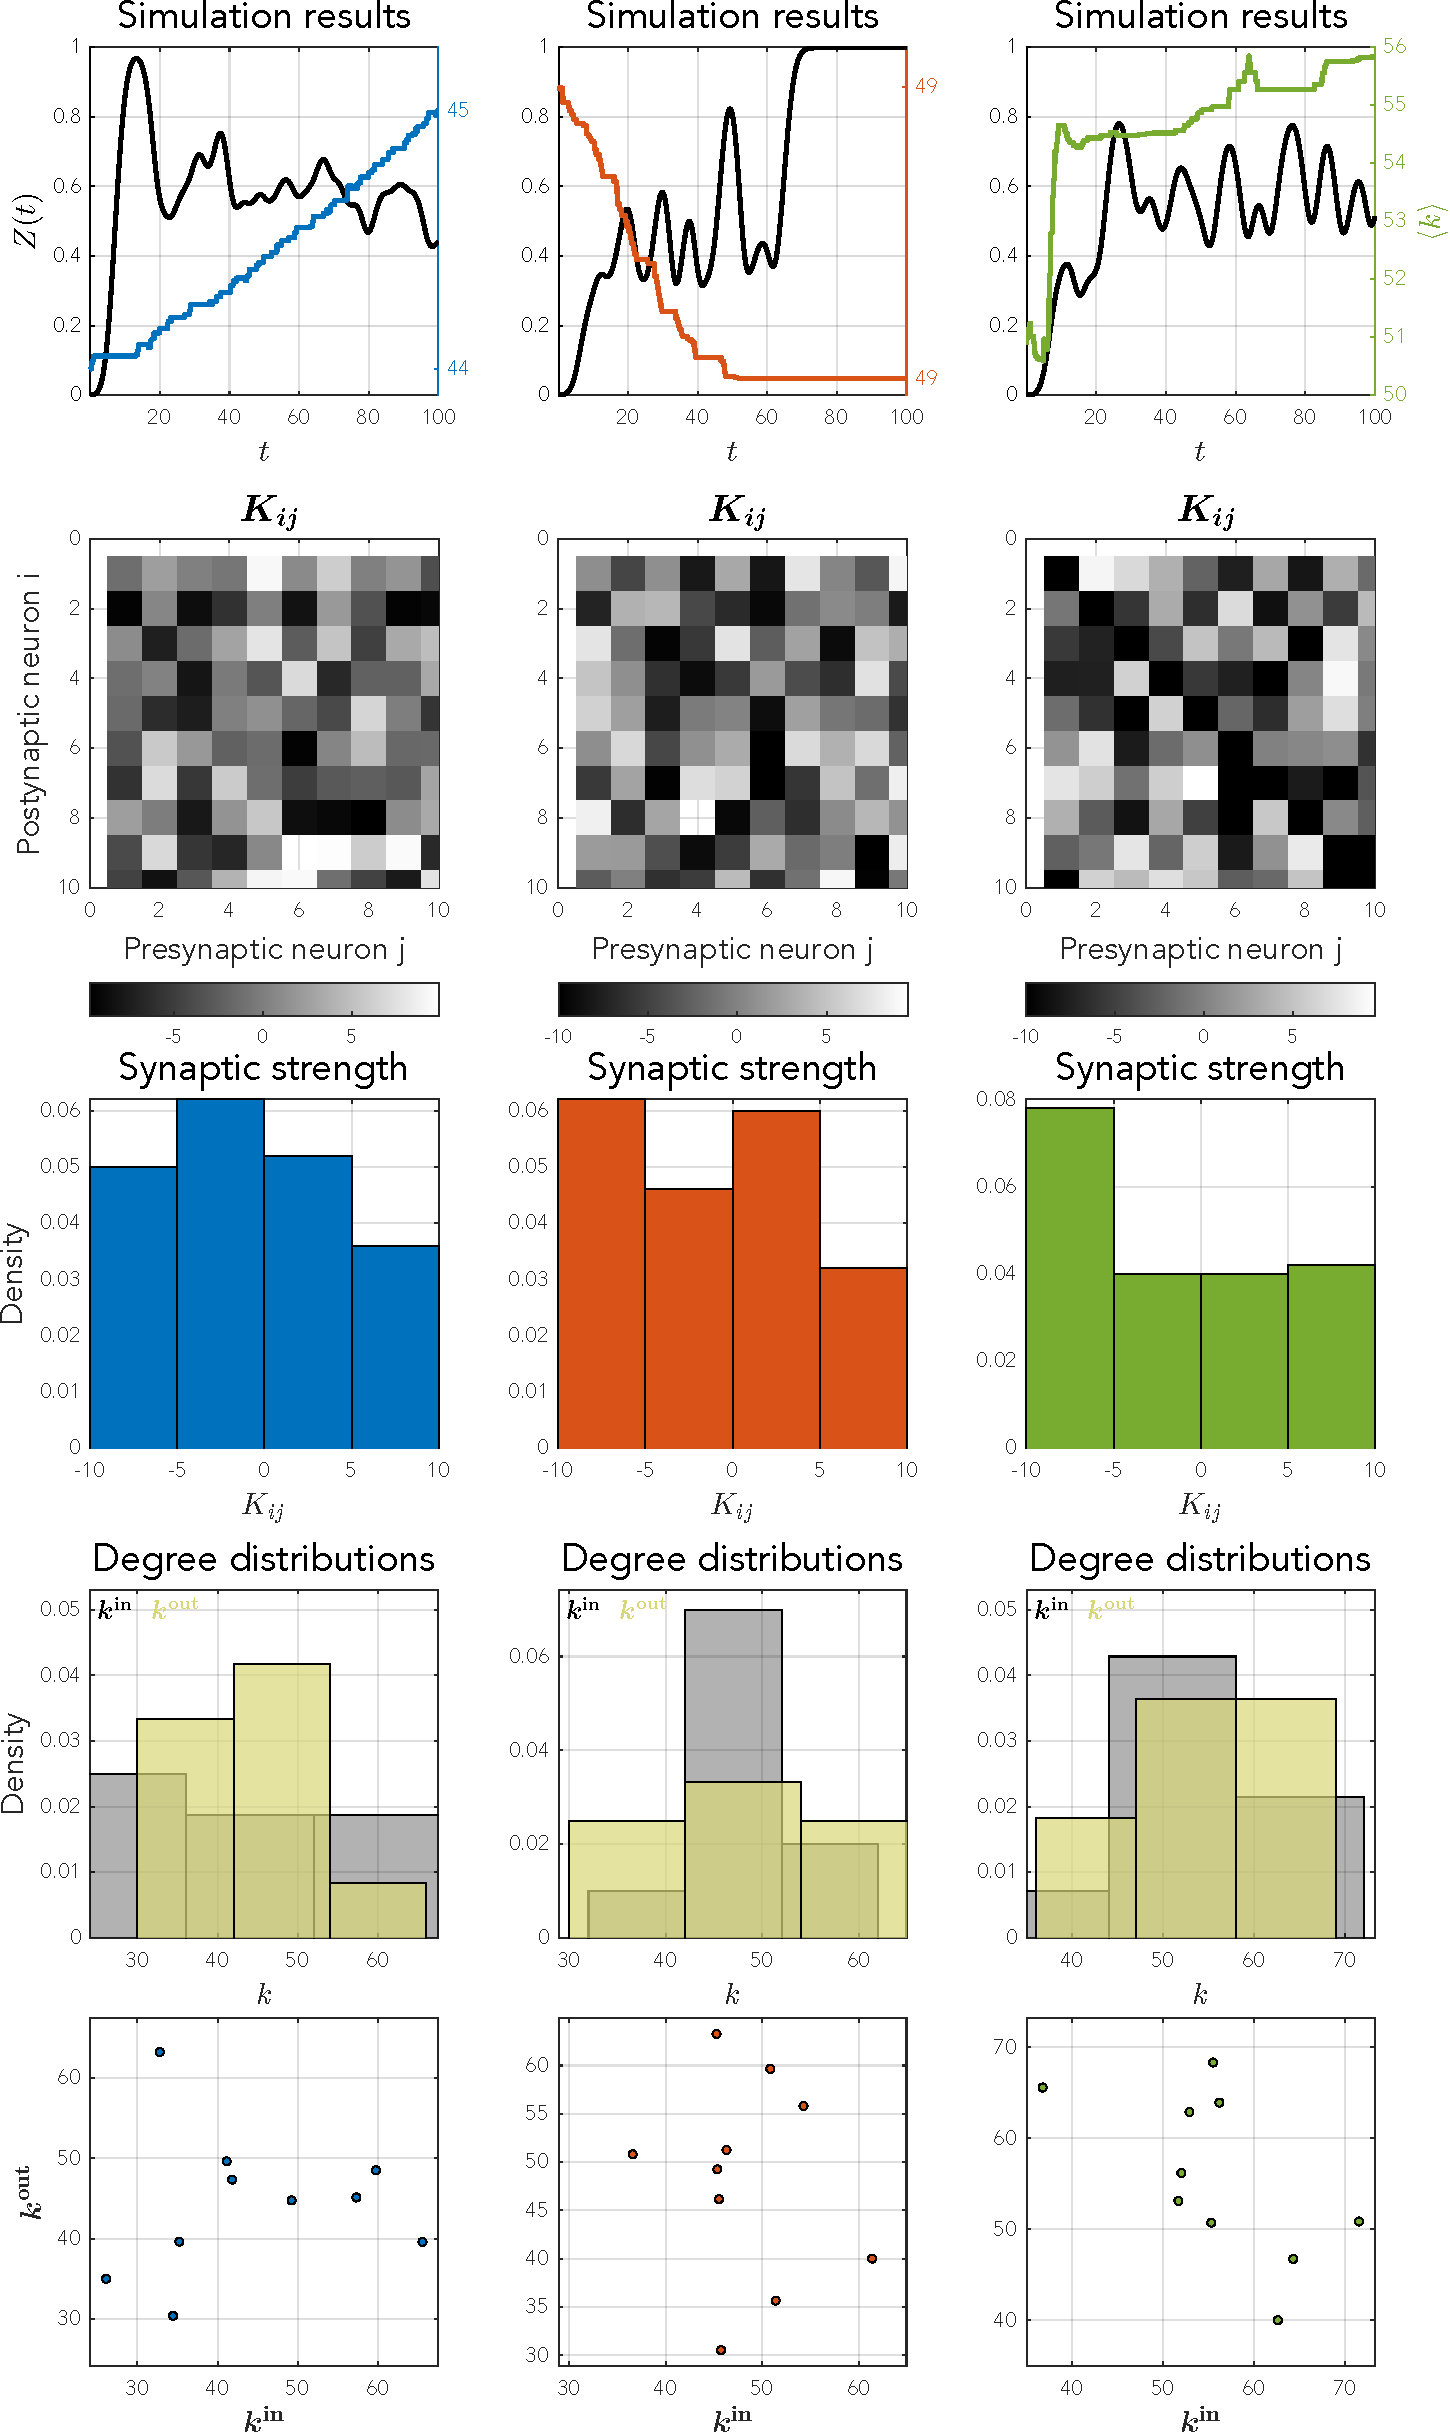
\includegraphics[height = \textheight]{../Figures/Learning/STDP.pdf}
\caption{Results of the \STDP learning.}
\label{fig:STDP}
\end{figure}

\begin{figure}[H]
\centering
\includegraphics[height = \textheight]{../Figures/Learning/STDPandIP.pdf}
\caption{Results of the \STDP learning with \IP learning.}
\label{fig:STDP}
\end{figure}

\subsection{Results}
\textcolor{red}{TODO}: \textsl{describe the emergent behaviour.}

